\documentclass{article}

%%% Packages: 
\usepackage{eurosym} % for euros symbol
\usepackage{amsfonts}
\usepackage{fancyhdr}
\usepackage[usenames,dvipsnames,svgnames,table]{xcolor}
\usepackage[hypertexnames=false]{hyperref} %This makes hyperref ``dumber'', and, hence, more robust! (otherwise sometimes the appendix links don't work).
\usepackage[pdftex]{graphicx}
\usepackage{amsmath, amsthm, amssymb, dsfont, amsfonts}
\usepackage[american]{babel}
\usepackage{color}
%\usepackage{subfig}
\usepackage{morefloats}
\usepackage{tabulary}
\usepackage{tabularx}
\usepackage{booktabs}
\usepackage{fullpage}
%\usepackage{bbm}
\usepackage{setspace}
\usepackage{float}
\usepackage{pdfpages}
\usepackage{lscape}
\usepackage{multirow}
\usepackage{array}
\usepackage{sectsty}
\usepackage{pdflscape}
\usepackage{placeins}
\usepackage[font={large,sc}]{caption}
\usepackage{comment}
\usepackage[margin=1in,headsep=.4in]{geometry}
\usepackage[normalem]{ulem}
\usepackage{natbib}
\usepackage{tikz}
\usepackage{tikzscale}
\usepackage{bibunits}
\usepackage{xr}
\usepackage[figuresright]{rotating}
\usepackage{subcaption}
\usepackage{caption}
\usepackage{makecell}
\usepackage{graphicx}
\usepackage{hyperref}
\usepackage{pdfpages}
\usepackage{afterpage}
\usepackage{eurosym}
\setcounter{MaxMatrixCols}{10}
\usepackage{ulem}
\renewcommand{\ULdepth}{1.8pt}

%%%%%%%%%%%%%%%%%%%%%%%%%%%%%%%%%%%%%%%%%%%%%%%%%%%%%%%%%
%% COLORS AND LINKS
\definecolor{dark-red}{rgb}{0.4,0.15,0.15}
\definecolor{dark-blue}{rgb}{0.15,0.15,0.4}
\definecolor{medium-blue}{rgb}{0,0,0.5}
\hypersetup{
 colorlinks, linkcolor={dark-red},
citecolor={dark-red}, urlcolor={dark-red}
}



%%%%%%%%%%%%%%%%%%%%%%%%%%%%%%%%%%%%%%%%%%%%%%%%%%%%%%%%%
%%% THEOREMS and PROPOSITIONS
\newtheorem{definit}{Definition}
\newtheorem{prop}{Proposition}
\newtheorem{cor}{Corollary}

\renewcommand{\topfraction}{0.9}
    \renewcommand{\bottomfraction}{0.8}
\setcounter{topnumber}{2}
\setcounter{bottomnumber}{2}
\setcounter{totalnumber}{4}
\setcounter{dbltopnumber}{2}
    \renewcommand{\dbltopfraction}{0.9}
    \renewcommand{\textfraction}{0.07}
    \renewcommand{\floatpagefraction}{0.7}
    \renewcommand{\dblfloatpagefraction}{0.7}

\newcommand{\sym}[1]{{#1}}

%%%%% PAGE LAYOUT 
\textwidth 6.5in
\textheight 8.84in
\setlength{\topmargin}{-0.3in}
\setlength{\oddsidemargin}{0.0in}
\setlength{\evensidemargin}{0.0in}
\setlength{\abovecaptionskip}{0pt}
\setlength{\belowcaptionskip}{5pt}
\setlength{\textfloatsep}{25pt}
\setlength{\intextsep}{5pt}

\captionsetup[table]{skip=-10pt}

%%%%%%%%%%%%%%%%%%%%%%%%%%%%%%%%%%%%%%%%%%%%%%%%%%%%%%%%%%%%%%%%%%
%%%%% TIKZ
\usetikzlibrary{er, positioning,decorations.pathmorphing,calc}
\tikzset{every entity/.style={draw=black, fill=white}}
\tikzset{comment/.style={draw=white, fill=white}}
%%%%%%%%%%%%%%%%%%%%%%%%%%%%%%%%%%%%%%%%%%%%%%%%%%%%%%%%%%%%%%%%%%


%%%%%%%%%%%%%%%%%%%%%%%%%%%%%%%%%%%%%%%%%%%%%%%%%%%%%%%%%%%%%%%%%% BIBLIOGRAPHY

%\bibliographystyle{chicago}




\usepackage[utf8]{inputenc}

\title{LDA method description}
\date{March 2021}

\begin{document}

\maketitle

\section{Selected Questions}
\begin{flushleft}
\textbf{a. Climate Knowledge}
\end{flushleft}
\begin{itemize}
    \item Q1. How often do you think or talk with people about climate change?\\
    \textit{Almost never; Several times a year; Several times a month}
    \item Q2. In your opinion, is climate change real?\\
    \textit{Yes; No}
    \item Q3. (If ``Yes'' to 2.) What part of climate change do you think is due to human activity?\\
    \textit{None; A little; Some; A lot; Most}

    \item Q4. Do you agree or disagree with the following statement: ``Climate change is an important problem.''\\
    \textit{Strongly disagree; Somewhat disagree; Neither agree nor disagree; Somewhat agree; Strongly agree}
    \item Q5. How knowledgeable do you consider yourself about climate change?\\
    \textit{Not at all; A little; Moderately; A lot; A great deal}
    \item Q6. Greenhouse gases are gases that trap heat in the atmosphere and make the Earth warmer, causing climate change. In particular, the burning of fossil fuels and agricultural production emit greenhouse gases.
    Which of the following elements contribute to climate change? (Multiple answers are possible) \\
    \textit{CO2; Hydrogen; Methane; Particulate matter}
    \item Q7. Do you think that cutting global greenhouse gas emissions by half would be sufficient to eventually stop temperatures from rising? \\
    \textit{Yes; No}

    For the next three questions we would like you to rank the items according to the greenhouse gas emissions they emit, to the best of your knowledge (where 1 is the item that emits the most and 3 the item that emits the least).
    The greenhouse gas emissions of a product are those emitted at all steps involved in its production and distribution.
    \item Q8. If a family of 4 travels 700 km from London to Glasgow, with which mode of transportation do they emit the most greenhouse gases?
    Please rank the items from 1 (most) to 3 (least) (by clicking and dragging the items).\\
    \textit{Car (running on diesel or gasoline); Train; Plane}
    \item Q9. Which dish emits the most greenhouse gases? We consider that each dish weighs half a pound.
    Please rank the items from 1 (most) to 3 (least) (by clicking and dragging the items).\\
    \textit{A beef steak; One serving of paste; Chicken wings}
    \item Q10. Which source of electric energy emits the most greenhouse gases to provide power for a house?
    Please rank the items from 1 (most) to 3 (least) (by clicking and dragging the items).\\
    \textit{Gas-fired power plant; Nuclear power plant; Coal-fired power station}
    \item QX. Which region contributes most to global greenhouse gas emissions? Please rank the regions from 1 (most) to 4 (least) and note that multiple regions may have the same rank.
        \begin{itemize}
            \item The U.S.
            \item The European Union
            \item China
            \item India
        \end{itemize}
    \textit{1; 2; 3; 4}
    \item Q11. Consider now per capita emissions: in which region does the consumption of an average person contribute most to greenhouse gas emissions?
    Please rank the regions from 1 (most) to 5 (least).
        \begin{itemize}
            \item The U.S.
            \item The European Union
            \item China
            \item India
            \item The U.K.
        \end{itemize}
    \textit{1; 2; 3; 4; 5}
    \item Q12. If nothing is done to limit climate change, how likely do you think it is that climate change will lead to the following events?
        \begin{itemize}
            \item Severe droughts and heatwaves
            \item More frequent volcanic eruptions
            \item Rising sea levels
            \item Lower agricultural production
            \item Drop in standards of living
            \item Larger migration flows
            \item More armed conflicts
            \item Extinction of humankind
        \end{itemize}
    \textit{Very unlikely; Somewhat unlikely; Somewhat likely; Very likely}
\end{itemize}

\begin{flushleft}
\textbf{b. Climate Attitudes}
\end{flushleft}

\begin{itemize}
    \item Q1. To what extent are the following groups responsible for climate change in the U.S.?
        \begin{itemize}
            \item Each of us
            \item The high income earners
            \item The UK government
            \item Companies
            \item Previous generations
        \end{itemize}
    \textit{Not at all; A little; Moderately; A lot; A great deal}
    \item Q2. To what extent do you think that it is technically feasible to stop greenhouse gas emissions by the end of the century while maintaining satisfactory standards of living in the UK?\\
    \textit{Not at all; A little; Moderately; A lot; A great deal}
    \item Q3. To what extent do you think climate change already affects or will affect your personal life negatively? \\
    \textit{Not at all; A little; Moderately; A lot; A great deal}
    \item Q4. How likely is it that human kind halt climate change by the end of the century? \\
    \textit{Very unlikely; Somewhat unlikely; Somewhat likely; Very likely}
    \item Q5. If we decide to halt climate change through ambitious policies, what would be the effects on the UK economy and employment? \\
    \textit{Very negative effects; Somewhat negative effects; No noticeable effects; Somewhat positive effects; Very positive effects}
    \item Q6. If we decide to halt climate change through ambitious policies to what extent do you think it would negatively affect your lifestyle? \\
    \textit{Not at all; A little; Moderately; A lot; A great deal}
    \item Q7. To what extent would you be willing to adopt the following behaviors? \\
    \textit{Limit flying/Limit driving/Electric vehicle/Limit beef/ Limit heating or cooling}
    \item Q8. Here are possible behaviors that experts say would help reduce greenhouse gas emissions.
    To what extent would you be willing to adopt the following behaviors?
        \begin{itemize}
            \item Limit flying
            \item Limit driving
            \item Have an electric vehicle
            \item Limit beef consumption
            \item Limit heating or cooling your home
        \end{itemize}
    \textit{Not at all; A little; Moderately; A lot; A great deal}
    \item Q9. How important are the factors below in order for you to adopt a sustainable lifestyle (i.e. limit driving, flying, and consumption, cycle more, etc.)?
        \begin{itemize}
            \item Ambitious climate policies
            \item Having enough financial support
            \item People around you also changing their behavior
            \item The most well-off also changing their behavior
        \end{itemize}
    \textit{Not at all; A little; Moderately; A lot; A great deal}
\end{itemize}
\begin{flushleft}
\textbf{c. Pref1: Ban on the sale of combustion-engine cars}
\end{flushleft}

\begin{itemize}
    \item Q1. Do you agree or disagree with the following statements? A ban on combustion-engine cars would...
    \begin{itemize}
        \item reduce $CO_2$ emissions from cars
        \item reduce air polution
        \item have a large effect on the UK economy and employment
        \item have a negative/positive effect on the UK economy and employment
        \item be a costly way to fight climate change
    \end{itemize}
    \textit{Strongly disagree; Somewhat disagree; Neither agree nor disagree; Somewhat agree; Strongly agree}
    \item Q2. In your view, would the following groups win or lose if a ban on combustion-engine cars was implemented in the UK?
    \begin{itemize}
    \item Low-income earners
    \item The middle class
    \item High-income earners
    \item Those living in rural areas
    \end{itemize}
    \textit{Lose a lot; Mostly lose; Neither win nor lose; Mostly win; Win a lot}
    \item Q3. Do you think that your household would win or lose financially from a ban on combustion-engine cars?  \\
    \textit{Lose a lot; Mostly lose; Neither win nor lose; Mostly win; Win a lot}
    \item Q4. Do you agree or disagree with the following statement: ``A ban on combustion-engine cars is fair''? \\
    \textit{Strongly disagree; Somewhat disagree; Neither agree nor disagree; Somewhat agree; Strongly agree}
    \item Q5. Do you support or oppose a ban on combustion-engine cars?
    \textit{Strongly oppose; Somewhat oppose; Neither support nor oppose; Somewhat support; Strongly support}
    \item Q6. Do you support or oppose a ban on combustion-engine cars where alternatives such as public transports are made available to people? \\
    \textit{Strongly oppose; Somewhat oppose; Neither support nor oppose; Somewhat support; Strongly support}
\end{itemize}

\begin{flushleft}
\textbf{d. Pref 2: Green infrastructure program}
\end{flushleft}

\begin{itemize}
    \item Q1. Do you agree or disagree with the following statements? A green infrastructure program would... 
    \begin{itemize}
        \item make electricity production greener
        \item increase the use of public transport
        \item reduce air polution
        \item have a large effect on the UK economy and employment
        \item have a negative/positive effect on the UK economy and employment
        \item be a costly way to fight climate change
    \end{itemize}
    \textit{Strongly disagree; Somewhat disagree; Neither agree nor disagree; Somewhat agree; Strongly agree}
    \item Q2. In your view, would the following groups win or lose with a green infrastructure program?''
    \begin{itemize}
        \item Low-income earners
        \item The middle class
        \item High-income earners
        \item Those living in rural areas
    \end{itemize}
    \textit{Lose a lot; Mostly lose; Neither win nor lose; Mostly win; Win a lot}
    \item Q3. Do you think that your household would win or lose financially from a green infrastructure program? \\
    \textit{Lose a lot; Mostly lose; Neither win nor lose; Mostly win; Win a lot}
    \item Q4. Do you agree or disagree with the following statement: ``A green infrastructure program is fair''? \\
    \textit{Strongly disagree; Somewhat disagree; Neither agree nor disagree; Somewhat agree; Strongly agree}
    \item Q5. Do you support or oppose a green infrastructure program? \\
    \textit{Strongly oppose; Somewhat oppose; Neither support nor oppose; Somewhat support; Strongly support}
    \item Q6. Until now, we have considered that a green infrastructure program would be financed by public debt, but other sources of funding are possible.
    What sources of funding do you find appropriate for public investments in green infrastructure? (Multiple answers are possible) \\
    \textit{Additional public debt; Increase in the VAT (value-added tax); Increase in taxes on the wealthiest; Reduction in social spending; Reduction in military spending}   
\end{itemize}

\begin{flushleft}
\textbf{e. Pref 3: Carbon tax with cash transfers}
\end{flushleft}

\begin{itemize}
    \item Q1. Do you agree or disagree with the following statements? A carbon tax with cash transfers would... 
    \begin{itemize}
        \item encourage people to drive less
        \item encourage people and companies to insulate buildings
        \item reduce the use of fossil fuels and greenhouse gas emissions
        \item reduce air polution
        \item have a large effect on the UK economy and employment
        \item have a negative/positive effect on the UK economy and employment
        \item be a costly way to fight climate change
    \end{itemize}
    \textit{Strongly disagree; Somewhat disagree; Neither agree nor disagree; Somewhat agree; Strongly agree}
    \item Q2. In your view, would the following groups win or lose under a carbon tax with cash transfers?
    \begin{itemize}
        \item Low-income earners
        \item The middle class
        \item High-income earners
        \item Those living in rural areas
    \end{itemize}
    \textit{Lose a lot; Mostly lose; Neither win nor lose; Mostly win; Win a lot}
    \item Q3. Do you think that your household would win or lose financially under a carbon tax with cash transfers? \\
    \textit{Lose a lot; Mostly lose; Neither win nor lose; Mostly win; Win a lot}
    \item Q4. Do you agree or disagree with the following statement: ``A carbon tax with cash transfers is fair.'' \\
    \textit{Strongly disagree; Somewhat disagree; Neither agree nor disagree; Somewhat agree; Strongly agree}
    \item Q5. Do you support or oppose a carbon tax with cash transfers? \\
    \textit{Strongly oppose; Somewhat oppose; Neither support nor oppose; Somewhat support; Strongly support}
    \item Q6. Now, we consider a variant of the policy where the cash transfers are higher for low-income people compared to high-income people. \\
    Do you agree or disagree that such a policy would be fair?
    \textit{Strongly disagree; Somewhat disagree; Neither agree nor disagree; Somewhat agree; Strongly agree}
    \item Q7. Do you support or oppose a carbon tax with cash transfers with higher transfers for low-income people compared to high-income people? \\
    \textit{Strongly oppose; Somewhat oppose; Neither support nor oppose; Somewhat support; Strongly support}
\end{itemize}

\begin{flushleft}
\textbf{f. Pref for Climate Policies}
\end{flushleft}

\begin{itemize}
    \item Q1. Do you support or oppose the following climate policies?
    \begin{itemize}
        \item A tax on flying (that increases ticket prices by 20\%)
        \item A national tax on fossil fuels (increasing gasoline prices by 8 cents per liter)
        \item A ban of polluting vehicles in dense areas, like city centers
        \item Subsidies for low-carbon technologies (renewable energy, capture and storage of carbon…)
        \item A contribution to a global climate fund to finance clean energy in low-income countries
    \end{itemize}
    \textit{Strongly oppose; Somewhat oppose; Neither support nor oppose; Somewhat support; Strongly support}
    \item Q2. Governments can use the revenues from carbon taxes in different ways. Would you support or oppose introducing a carbon tax that would raise gasoline prices by 8 cents per liter, if the government used this revenue to finance...
    \begin{itemize}
    \item Cash transfers to households with no alternative to using fossil fuels
    \item Cash transfers to the poorest households
    \item Equal cash transfers to all households
    \item A reduction in personal income taxes
    \item A reduction in corporate income taxes
    \item Tax rebates for the most affected firms
    \item Funding environmental infrastructure projects (public transport, cycling ways, etc.)
    \item Subsidize low-carbon technologies, including renewable energy
    \item A reduction in the public deficit
    \end{itemize}
    \textit{Strongly oppose; Somewhat oppose; Neither support nor oppose; Somewhat support; Strongly support}
\end{itemize}


\begin{flushleft}
\textbf{h. Willingness to Pay and real stake questions}
\end{flushleft}

\begin{itemize}
    \item Q1. Are you willing to pay (£10 / £30 / £50 / £100 / £300 /£500 / £1,000) annually through an additional individual contribution to limit global warming to safe levels (less than 2 degrees Celsius)?  \\
    \textit{Yes; No}
    \item Q2. Should you win the lottery, please enter your donation amount using the slider below: \\
    \textit{Slide going from 0 to 100}
\end{itemize}

\begin{flushleft}
\textbf{h. International Burden-Sharing}
\end{flushleft}

\begin{itemize}
    \item Q1. At which level(s) do you think public policies to tackle climate change need to be put in place? (Multiple answers are possible)  \\
    \textit{Global; European; National; Local}
    \item Q2. Do you agree or disagree with the following statement: ``The UK should take measures to fight climate change.'' \\
    \textit{Strongly disagree; Somewhat disagree; Neither agree nor disagree; Somewhat agree; Strongly agree}
    \item Q3. How should UK climate policies depend on what other countries do?
    \begin{itemize}
        \item If other countries do more, the UK should do… 
        \item If other countries do less, the UK should do…
    \end{itemize}
    \textit{Much less; Less; About the same; More; Much more}
    \item Q4. To achieve a given reduction of greenhouse gas emissions globally, costly investments are needed.
    Ideally, how should countries bear the costs of fighting climate change?
    \begin{itemize}
        \item Countries should pay in proportion to their income
        \item Countries should pay in proportion to their current emissions
        \item Countries should pay in proportion to their past emissions (from 1990 onwards)
        \item The richest countries should pay it all, so that the poorest countries do not have to pay anything
        \item The richest countries should pay even more, to help vulnerable countries face adverse consequences: vulnerable countries would then receive money instead of paying
    \end{itemize}
    \textit{Strongly disagree; Somewhat disagree; Neither agree nor disagree; Somewhat agree; Strongly agree}
    \item Q5. Do you support or oppose establishing a global democratic assembly whose role would be to draft international treaties against climate change? Each adult across the world would have one vote to elect members of the assembly.  \\
    \textit{Strongly oppose; Somewhat oppose; Neither support nor oppose; Somewhat support; Strongly support}
    \item Q6. Imagine the following policy: a global tax on greenhouse gas emissions funding a global basic income.
    Such a policy would progressively raise the price of fossil fuels (for example, the price of gasoline would increase by 8 cents per liter in the first years). Higher prices would encourage people and companies to use less fossil fuels, reducing greenhouse gas emissions. Revenues from the tax would be used to finance a basic income of \$30 (or £22) per month to each human adult, thereby lifting the 700 million people who earn less than \$2/day out of extreme poverty.
    The average British person would lose a bit from this policy as they would face £42 per month in price increases, which is higher that the £22 they would receive. \\
    Do you support or oppose such a policy?  \\
    \textit{Strongly oppose; Somewhat oppose; Neither support nor oppose; Somewhat support; Strongly support}
    \item Q7. Do you support or oppose a tax on all millionaires around the world to finance low-income countries that comply with international standards regarding climate action?  \\
    \textit{Strongly oppose; Somewhat oppose; Neither support nor oppose; Somewhat support; Strongly support}
\end{itemize}

\begin{flushleft}
\textbf{i. Housing and cattle products}
\end{flushleft}

\begin{itemize}
    \item Q1. (If ``Owner'' or ``Landlord renting out'' at Background Questions 18.) How likely is it that you will improve the insulation or replace the heating system of your accommodation over the next 5 years?
    \textit{Very unlikely; Somewhat unlikely; Somewhat likely; Very likely}
    \item Q2. (If ``Owner'' or ``Landlord renting out'' at Background Questions 18.) What are the main hurdles preventing you from improving the insulation or replace the heating system of your accommodation? (Multiple answers are possible)
    \textit{The choice to insulate or replace the heating system is not mine; The upfront costs are too high; It is too much effort; It won't improve its energy efficiency; My insulation and heating systems are already satisfactory}
    \item Q3. GROUP 1.
    Imagine that the UK government makes it mandatory for all residential buildings to have insulation that meets a certain energy efficiency standard before 2040. The government would subsidise half of the insulation costs to help households with the transition. 
    Do you support or oppose such policy? \\
    GROUP 2. Imagine that the UK government makes it mandatory for all residential buildings to have insulation that meets a certain energy efficiency standard before 2040. The government would subsidise half of the insulation costs to help households with the transition.
    Insulating your home can take long, may cause disruptions to your daily life during the renovation works, and may even require you to leave your home until the renovation is completed.
    Do you support or oppose such policy? 
    \textit{Strongly oppose; Somewhat oppose; Neither support nor oppose; Somewhat support; Strongly support}
    \item Q4. Imagine that, in order to fight climate change, the UK government decides to limit the consumption of cattle products like beef and dairy.
    Do you support or oppose the following options?
    \begin{itemize}
        \item A high tax on cattle products, so that the price of beef doubles
        \item Subsidies on organic and local vegetables, fruits, and nuts
        \item The removal of subsidies for cattle farming
        \item The ban of intensive cattle farming
    \end{itemize}
    \textit{Strongly oppose; Somewhat oppose; Neither support nor oppose; Somewhat support; Strongly support}
\end{itemize}

\begin{flushleft}
\textbf{j. Trust, Perceptions of Institutions, Inequality, and the Future}
\end{flushleft}

\begin{itemize}
    \item Q1. Do you agree or disagree with the following statement: ``Most people can be trusted.''
    \textit{Strongly disagree; Somewhat disagree; Neither agree nor disagree; Somewhat agree; Strongly agree}
    \item Q2. Do you agree or disagree with the following statement: ``Over the last decade the UK government could generally be trusted to do what is right.''
    \textit{Strongly disagree; Somewhat disagree; Neither agree nor disagree; Somewhat agree; Strongly agree}
    \item Q3. Some people think the government is trying to do too many things that should be left to individuals and businesses. Others think that government should do more to solve our country's problems. Which come closer to your own view?
    \textit{Government is doing too much; Government is doing just the right amount; Government should do more}
    \item Q4. How big of an issue do you think income inequality is in the UK?
    \textit{Not an issue at all; A small issue; An issue; A serious issue; A very serious issue}
    \item Q5. Do you think that overall people in the world will be richer or poorer in 100 years from now?
    \textit{Much poorer; Poorer; As rich as now; Richer; Much richer}
\end{itemize}

\begin{flushleft}
\textbf{k. Feedback}
\end{flushleft}

\begin{itemize}
    \item Q1. Do you feel that this survey was politically biased?
    \textit{Yes, left-wing biased; Yes, right-wing biased; No, I do not feel it was biased}
\end{itemize}

\begin{flushleft}
\textbf{l. Petition}
\end{flushleft}

\begin{itemize}
    \item Q1. Finally, are you willing to sign a petition to ``stand up for real climate action''?
    As soon as the survey is complete, we will send the results to the Prime Minister's office, informing him what share of people who took this survey were willing to support the following petition. 
    ``I agree that immediate action on climate change is critical. Now is the time to dedicate ourselves to a low-carbon future and prevent lasting damage to all living things. Science shows us we cannot afford to wait to cut harmful carbon emissions. I'm adding my voice to the call to world leaders in the UK and beyond -- to act so we do not lose ground in combating climate change.''
    Do you support this petition (you will NOT be asked to sign, only your answer here is required and remains anonymous)? 

    \textit{Yes; No}
\end{itemize}

\section{Top answers per profile}
Percentages in brackets are the entries of the $\beta$ vector scaled-up following methodology from \cite{draca2020polarized}. Therefore they correspond to the probability of an answer to appear for a given profile.
\subsection{Two Profiles}

\textbf{Profile 1 : X}

\begin{itemize}
    \item ``An emission limit for cars would reduce $CO_2$ emissions from cars.'' [\textit{79.2\%}]
    \item ``An emission limit for cars would reduce air pollution.'' [\textit{78.9\%}]
    \item ``A green infrastructure program would reduce air pollution.'' [\textit{77.9\%}]
    \item ``The U.S. should take measures to fight climate change.'' [\textit{77.9\%}]
    \item ``A carbon tax with cash transfers would reduce air pollution.'' [\textit{76.6\%}]
    \item ``A green infrastructure program would make electricity production greener.'' [\textit{76.4\%}]
\end{itemize}

\textbf{Profile 2 : X}
\begin{itemize}
   \item ``Funding a green infrastructure program with public debt is not appropriate.'' [\textit{76.5\%}]
   \item ``Funding a green infrastructure program with a reduction in military spending is not appropriate.'' [\textit{75.1\%}]
   \item ``Disagree that over the last decade the U.S. federal government could generally be trusted to do what is right.'' [\textit{66.3\%}]
   \item ``It is unlikely that human kind halt climate change by the end of the century.'' [\textit{65.8\%}]
   \item ``Public policies to tackle climate change should not be put in place at the State level.'' [\textit{65.0\%}]
   \item ``Oppose a high tax on cattle products.'' [\textit{64.6\%}]
\end{itemize}



\subsection{Three Profiles}

\textbf{Profile 1 : X}

\begin{itemize}
    \item ``Support an emission limit for cars.'' [\textit{78.6\%}] 
    \item ``A carbon tax with cash transfers would encourage people and companies to insulate buildings.'' [\textit{78.3\%}]
    \item ``A carbon tax with cash transfers would reduce the use of fossil fuels.'' [\textit{78.2\%}]
    \item ``Support a policy where the U.S. federal government would make it mandatory for all residential buildings to have insulation that meets a certain energy efficiency standard before 2040 and would subsidize half of it.'' [\textit{78.2\%}]
    \item ``Support a carbon tax, if the government uses this revenue for funding environmental infrastructure projects.'' [\textit{77.9\%}]
    \item ``Support a green infrastructure program.'' [\textit{77.4\%}]
\end{itemize}

\textbf{Profile 2 : X}
\begin{itemize}
\item ``Climate change is real.'' [\textit{81.4\%}]
\item ``Funding a green infrastructure program with an increase in taxes on the wealthiest is appropriate.'' [\textit{79.5\%}]
\item ``Funding a green infrastructure program with an increase in sales taxes is not appropriate.'' [\textit{78.1\%}]
\item ``The middle class would neither win nor lose if an emission limit for cars was implemented.'' [\textit{76.8\%}]
\item ``My househould would neither win nor lose financially from an emission limit for cars.'' [\textit{76.3\%}]
\item ``The middle class would neither win nor lose with a green infrastructure program.'' [\textit{74.7\%}]
\end{itemize}

\textbf{Profile 3 : X}
\begin{itemize}
\item ``Funding a green infrastructure program with public debt is not appropriate.'' [\textit{87.7\%}]
\item ``Disagree that over the last decade the U.S. federal government could generally be trusted to do what is right.'' [\textit{85.2\%}]
\item ``Oppose a high tax on cattle products.'' [\textit{83.9\%}]
\item ``Disagree that the richest countries should pay it all, so that the poorest countries do not have to pay anything.'' [\textit{79.1\%}]
\item ``Funding a green infrastructure program with a reduction in military spending is not appropriate.'' [\textit{78.9\%}]
\item ``Oppose a national tax on fossil fuels (increasing gasoline prices by 40cts per gallon)'' [\textit{77.5\%}]
\end{itemize}

\subsection{Four Profiles}

\textbf{Profile 1 : X}
\begin{itemize}
\item ``Support a green infrastructure program.'' [\textit{90.5\%}]
\item ``An emission limit for cars would be cost-effective to fight climate change.'' [\textit{89.3\%}]
\item ``Support an emission limit for cars where alternatives such as public transports are made available to people.'' [\textit{89.3\%}]
\item ``Support establishing a global democratic assembly.'' [\textit{88.0\%}]
\item ``Support a contribution to a global climate fund to finance clean energy in low-income countries.'' [\textit{87.6\%}]
\item ``A green infrastructure program would be cost-effective to fight climate change.'' [\textit{85.7\%}]
\end{itemize}


\textbf{Profile 2 : X}
\begin{itemize}
\item ``The middle class would neither win nor lose if an emission limit for cars was implemented.'' [\textit{82.9\%}] 
\item `The middle class would neither win nor lose with a green infrastructure program.'' [\textit{81.2\%}]
\item ``My househould would neither win nor lose financially with a green infrastructure program.'' [\textit{80.4\%}]
\item ``My househould would neither win nor lose financially from an emission limit for cars.'' [\textit{80.1\%}]
\item ``My househould would neither win nor lose financially under a carbon tax with cash transfers.'' [\textit{80.1\%}]
\item ``People living in rural areas would neither win nor lose if an emission limit for cars was implemented.'' [\textit{79.0\%}]
\end{itemize}

\textbf{Profile 3 : X}
\begin{itemize}
\item ``Oppose a high tax on cattle products.'' [\textit{88.2\%}]
\item ``Oppose a national tax on fossil fuels (increasing gasoline prices by 40cts per gallon)'' [\textit{82.6\%}]
\item ``Not willing to limit heating or cooling her home.'' [\textit{82.0\%}]
\item ``Oppose the ban of intensive cattle farming.'' [\textit{79.0\%}]
\item ``It is unlikely that human kind halt climate change by the end of the century.'' [\textit{78.8\%}]
\item ``Oppose the removal of subsidies for cattle farming'' [\textit{78.6\%}]
\end{itemize}

\textbf{Profile 4 : X}
\begin{itemize}
\item ``An emission limit for cars would reduce $CO_2$ emissions from cars.'' [\textit{96.4\%}]
\item ``An emission limit for cars would reduce air pollution.'' [\textit{96.1\%}]
\item ``The U.S. should take measures to fight climate change.'' [\textit{96.0\%}]
\item ``A green infrastructure program would reduce air pollution.'' [\textit{95.4\%}]
\item ``Companies are a lot responsible for climate change in the U.S..'' [\textit{94.9\%}]
\item ``Support mandatory insulation of buildings'' [\textit{94.4\%}]
\end{itemize}

\section{Optimal Number of Profiles}
We assess the cohesion of models using the cohesion measure developed by \cite{draca2020polarized}. They use the Normalized Pointwise Mutual Information (NPMI) \citep{bouma2009normalized} (which captures the frequence at which two features appear together on a $[-1,1]$ scale). The NPMI are averaged over the $B$ most important positions of a profile. Finally the cohesion of a model is defined as the average of the overall NPMI of each profile.
As in \cite{lau2016sensitivity} the measure of cohesion is calculated for different number of features $B \in (5,10,15,20)$. Similarly to \cite{draca2020polarized}, the 4 type LDA specification performs best.

\begin{figure}[h!]
\caption{Average Cohesion of Profiles for Different LDA Models}
\begin{center}
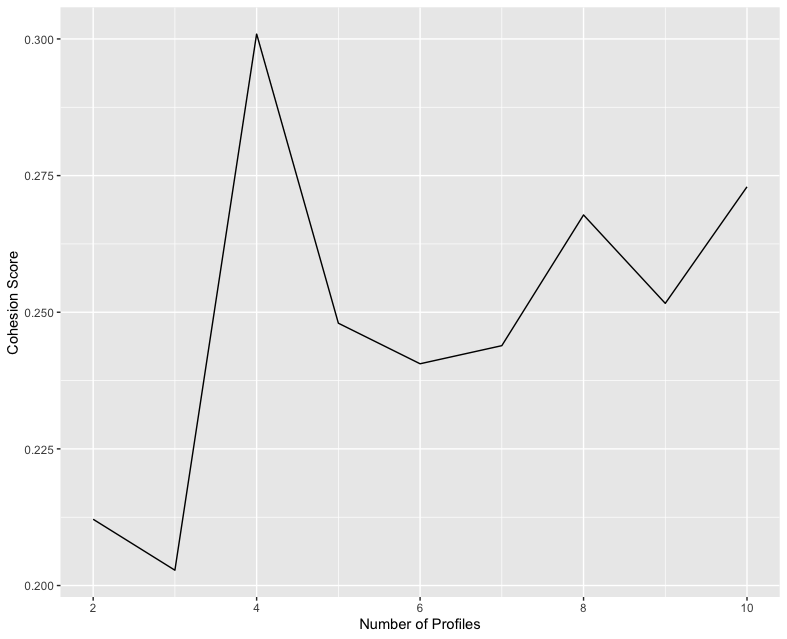
\includegraphics[width=.8\textwidth]{cohesion_score.png}
\end{center}
{\footnotesize Note: Cohesion scores for models with $M \in [\![2,10]\!]$. Topic cohesion is calculated as the average cohesion for score for features $B \in (5,10,15,20)$.}
\end{figure}


\begin{figure}[h!]
\caption{Average Cohesion from \cite{draca2020polarized}}
\begin{center}
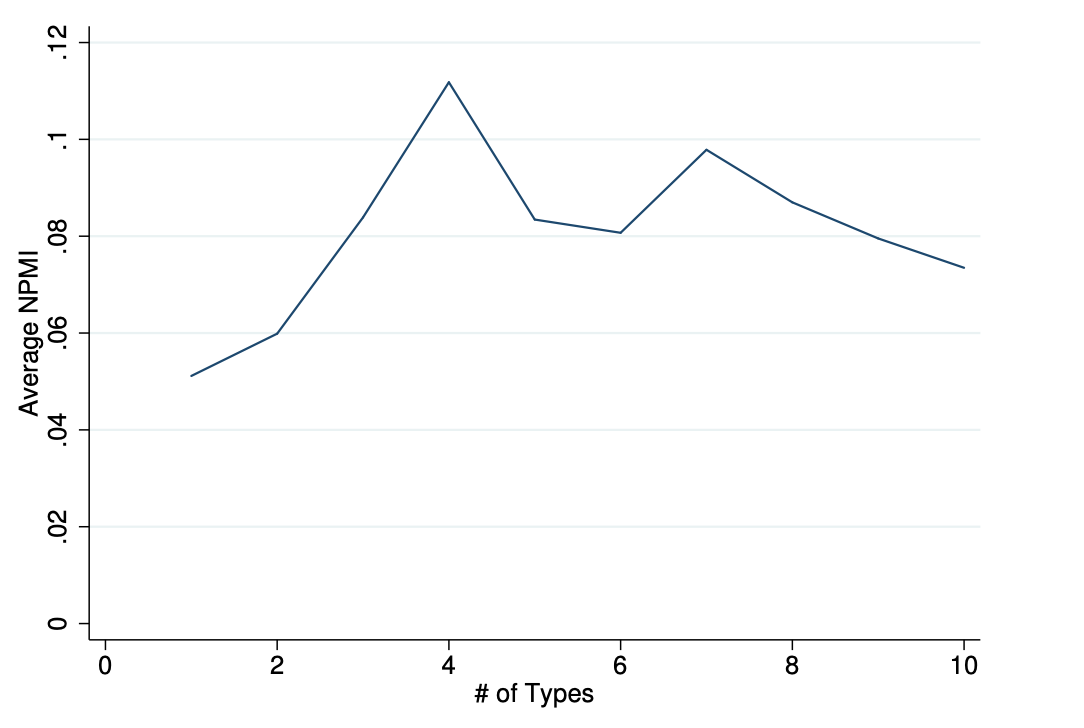
\includegraphics[width=.8\textwidth]{cohesion_score_draca_schwarz.png}
\end{center}
\end{figure}

\clearpage

\section{Regressions}
\begin{table}[h!]
    \caption{2-profiles}
    \begin{center}
        \scalebox{0.7}{\input{"topic2.tex"}}
    \end{center}
    {\footnotesize Note: The dependent variables are indicator variables equal to one if the respondent has been assigned to this profile (generally because most of her responses belong to this profile). 
    The \textit{race: White only} indicator variable equals one if the respondent's self reported race is only ``White." The regression includes controls for gender, having children and not having completed a college degree. The three \textit{status} indicator variables indicate the difference in mean compared to a reference group of people not working (either unemployed or inactive). The \textit{status: Working} indicator variable includes respondents who self-reported being either ``Full-time employed", ``Part-time employed", or ``Self-employed". The three \textit{Income} indicator variables indicate difference in mean compared to a reference group of people in the first quartile of household's annual income in 2019 (i.e. income $<$ \textdollar 35,000). The five \textit{age} indicator variables indicate difference in mean compared to a reference group of people aged between 18 and 24. The two \textit{vote} indicator variables indicate difference in mean compared to a reference group of people who either did not vote in the 2020 Presidential election or voted for another candidate than Biden or Trump.
    \newline  *p$<$0.1; **p$<$0.05; ***p$<$0.01}
\end{table} 

\begin{table}[h!]
    \caption{3-profiles}
    \begin{center}
        \scalebox{0.7}{\input{"topic3.tex"}}
    \end{center}
    {\footnotesize Note: The dependent variables are indicator variables equal to one if the respondent has been assigned to this profile (generally because most of her responses belong to this profile). 
    The \textit{race: White only} indicator variable equals one if the respondent's self reported race is only ``White." The regression includes controls for gender, having children and not having completed a college degree. The three \textit{status} indicator variables indicate the difference in mean compared to a reference group of people not working (either unemployed or inactive). The \textit{status: Working} indicator variable includes respondents who self-reported being either ``Full-time employed", ``Part-time employed", or ``Self-employed". The three \textit{Income} indicator variables indicate difference in mean compared to a reference group of people in the first quartile of household's annual income in 2019 (i.e. income $<$ \textdollar 35,000). The five \textit{age} indicator variables indicate difference in mean compared to a reference group of people aged between 18 and 24. The two \textit{vote} indicator variables indicate difference in mean compared to a reference group of people who either did not vote in the 2020 Presidential election or voted for another candidate than Biden or Trump.
    \newline  *p$<$0.1; **p$<$0.05; ***p$<$0.01}
\end{table} 

\begin{table}[h!]
    \caption{4-profiles}
    \begin{center}
        \scalebox{0.7}{\input{"topic4.tex"}}
    \end{center}
    {\footnotesize Note: The dependent variables are indicator variables equal to one if the respondent has been assigned to this profile (generally because most of her responses belong to this profile). 
    The \textit{race: White only} indicator variable equals one if the respondent's self reported race is only ``White." The regression includes controls for gender, having children and not having completed a college degree. The three \textit{status} indicator variables indicate the difference in mean compared to a reference group of people not working (either unemployed or inactive). The \textit{status: Working} indicator variable includes respondents who self-reported being either ``Full-time employed", ``Part-time employed", or ``Self-employed". The three \textit{Income} indicator variables indicate difference in mean compared to a reference group of people in the first quartile of household's annual income in 2019 (i.e. income $<$ \textdollar 35,000). The five \textit{age} indicator variables indicate difference in mean compared to a reference group of people aged between 18 and 24. The two \textit{vote} indicator variables indicate difference in mean compared to a reference group of people who either did not vote in the 2020 Presidential election or voted for another candidate than Biden or Trump.
    \newline  *p$<$0.1; **p$<$0.05; ***p$<$0.01}
\end{table} 

\clearpage



\begin{spacing}{0.5}
\bibliographystyle{chicago}
\bibliography{My_Library}
\end{spacing}
\end{document}